% musicar-S-piano: the earlier solo-piano base (checkpoints/big_107M), drawn in the poster's style (architecture.tex).
% No captions, no instrument, learned positions. Teal = structure, grey = linear layers and embedding tables.
% Sources: shapes and parameter counts from checkpoints/big_107M/model_bf16.pt (model_args, state dict) and
% musicar/model/gpt.py (MusicEmbeddings, Block, CascadeHeads, ResidualHead); recipe from its stored config
% (config/pretrain/big.py) and logs/big_107M.log; result from context/claude/agents.md (2026-09-30 row).
% Build: pdflatex base_107m_piano.tex  (TinyTeX: export PATH=$HOME/.local/bin:$PATH)
% PNG / SVG: pdftoppm -r 200 -png -singlefile base_107m_piano.pdf base_107m_piano ; pdftocairo -svg base_107m_piano.pdf base_107m_piano.svg
\documentclass[border=8pt]{standalone}
% Shared preamble of the per-model diagrams (base_450m.tex, base_107m_band.tex, base_107m_piano.tex,
% base_models.tex): packages, colours, TikZ styles and macros copied unchanged from architecture.tex, so they look
% the same. Use after \documentclass[border=8pt]{standalone}; keep in sync when the poster's style changes.

\usepackage[T1]{fontenc}
\usepackage[scaled=0.92]{helvet}
\renewcommand{\familydefault}{\sfdefault}
\usepackage{inconsolata}
\usepackage{amsmath}
\usepackage[italic]{mathastext}     % maths letters and digits in Helvetica, like the text
\usepackage[table]{xcolor}
\usepackage{array}
\usepackage{tabularx}
\usepackage{pgfplots}
\pgfplotsset{compat=1.18}
\usepackage{tikz}
\usetikzlibrary{arrows.meta,calc,decorations.pathreplacing,backgrounds}
\usepackage[hidelinks]{hyperref}
\hyphenpenalty=10000
\exhyphenpenalty=10000

\definecolor{tealT}{HTML}{3B7D70}   % title, structure labels, section numbers, brace
\definecolor{tealF}{HTML}{C3E0D6}   % repeated block, table header
\definecolor{tealB}{HTML}{6FA696}
\definecolor{greyF}{HTML}{F2F2F2}   % containers, text panels
\definecolor{greyB}{HTML}{8A8A8A}
\definecolor{rowG}{HTML}{F2F2F2}    % alternating table rows
\definecolor{pinkL}{HTML}{C2577A}   % captions: lines, labels
\definecolor{pinkF}{HTML}{F6CCD9}
\definecolor{boxG}{HTML}{D5D5D5}    % linear layers, embedding tables
\definecolor{altG}{HTML}{767676}    % curves: the alternative a choice was compared with (teal = what the model uses)

\tikzset{
  box/.style={draw=black, fill=white, rounded corners=3pt, minimum height=5.6mm, inner sep=3pt, align=center,
              font=\footnotesize, line width=0.6pt},
  gbox/.style={box, fill=boxG},
  pbox/.style={box, fill=pinkF, draw=pinkL},
  sub/.style={draw=tealB, dashed, rounded corners=6pt, line width=0.9pt},
  sublab/.style={text=tealT, font=\footnotesize\bfseries},
  zoom/.style={draw=black, densely dotted, rounded corners=10pt, line width=1.5pt},
  zline/.style={densely dotted, line width=1.5pt},
  panel/.style={draw=greyB, fill=greyF, rounded corners=8pt, line width=1pt},
  ptitle/.style={font=\small\bfseries, anchor=south west, inner sep=2pt},
  arr/.style={-{Stealth[length=2.4mm]}, line width=0.9pt},
  parr/.style={arr, draw=pinkL},
  sum/.style={draw=black, fill=white, circle, inner sep=0pt, minimum size=4.6mm, line width=0.8pt},
  tok/.style={draw=black, fill=white, minimum width=2.9mm, minimum height=2.9mm, inner sep=0pt, line width=0.4pt},
  ptok/.style={tok, fill=pinkF, draw=pinkL},
  note/.style={font=\scriptsize, text=black!85, align=left},
  ptext/.style={font=\footnotesize, text=black!90, align=left, inner sep=8pt},
  head/.style={box, minimum width=9mm, minimum height=7.5mm, inner sep=1pt, densely dotted, line width=1.1pt},
}
\newcommand{\rcite}[1]{{\scriptsize[#1]}}
\newcommand{\capt}[1]{\textcolor{pinkL}{``#1''}}
\newcommand{\badge}[1]{\tikz[baseline=(b.base)]\node[circle, fill=tealT, text=white, inner sep=0pt, minimum size=4.4mm,
  font=\scriptsize\bfseries] (b) {#1};}
\newcommand{\sect}[2]{\badge{#1}\hspace{4pt}#2}

\pgfplotsset{cplot/.style={scale only axis, width=5.3cm, height=3.3cm, axis lines*=left, axis line style={black!55},
  tick style={black!55}, grid=major, grid style={black!10}, tick label style={font=\scriptsize}, label style={font=\scriptsize},
  every axis plot/.append style={line join=round}, clip=false, xlabel shift=-2pt, ylabel shift=-3pt,
  scaled ticks=false, tick label style={/pgf/number format/fixed}}}


\begin{document}
\newsavebox{\embBox}
\sbox{\embBox}{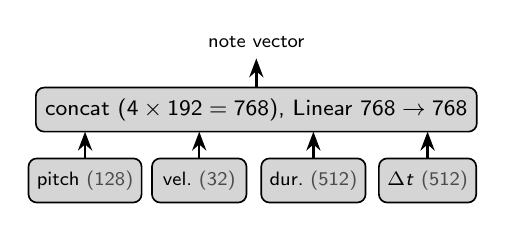
\begin{tikzpicture}
  \foreach \n/\v [count=\i] in {pitch/128, vel./32, dur./512, $\Delta t$/512} {
    \node[gbox, minimum width=12mm, font=\scriptsize] (e\i) at (1.45*\i, 0) {\n\ \textcolor{black!70}{(\v)}};
    \draw[arr] (e\i.north) -- (1.45*\i, 0.62);
  }
  \node[gbox, minimum width=56mm] (cat) at (3.625, 0.9) {concat ($4\times192 = 768$), Linear $768\to768$};
  \draw[arr] (cat.north) -- (3.625, 1.55) node[above, font=\scriptsize] {note vector};
\end{tikzpicture}}

\begin{tikzpicture}

%% ================= title =================
\node[font=\fontsize{20}{22}\selectfont\bfseries, text=tealT] at (4.35, 19.55) {musicar-S-piano (107M)};
\node[font=\footnotesize, text=black!85] at (4.35, 18.9) {106.84M parameters: trunk 99.11M, cascade heads 6.52M,
  embeddings 1.21M. Solo piano, context 512 notes.};
\node[font=\scriptsize, text=black!75, text width=17.3cm, align=center] at (4.35, 18.2) {How to read: numbers give the
  reading order; teal = the repeated block; grey boxes = linear layers and embedding tables; dashed frame = a module drawn
  open in place; dotted frame or box = a zoom (white panel) into the dotted part.};

%% ================= 1: main column =================
\node[ptitle] at (-4.3, 17.05) {\sect{1}{Music model}};
\begin{scope}[on background layer]
  \fill[greyF, draw=greyB, rounded corners=16pt, line width=1pt] (-4.3, -1.75) rectangle (4.3, 15.75);
  \fill[tealF, draw=tealB, rounded corners=12pt, line width=0.8pt] (-3.6, 3.45) rectangle (3.6, 11.35);
\end{scope}

% input
\node[box] (inp) at (0, -0.65) {Note tokens {\scriptsize (one position = one note: $\Delta t$, pitch, dur., vel.)}};
\node[font=\footnotesize, text=black!85] at (0, -1.35) {e.g. 512 notes of solo piano};
\draw[arr] (inp) -- (0, 0.67);

% embedding + learned position
\node[gbox, densely dotted, line width=1.1pt] (emb) at (0, 0.95) {Note embedding {\scriptsize ($4\times192$, concat, Linear)}};
\node[sum] (s0) at (0, 1.85) {$+$};
\node[gbox, densely dotted, line width=1.1pt, font=\scriptsize] (pos) at (2.45, 1.85) {Learned position\\[-1pt] (table $512\times768$)};
\draw[arr] (emb) -- (s0);
\draw[arr] (pos.west) -- (s0);

% input sequence: one vector per note, positions 0..511
\foreach \k in {-11,...,5} { \node[tok] at (0.32*\k, 2.85) {}; }
\node[font=\scriptsize] at (2.18, 2.85) {$\cdots$};
\node[tok] (last) at (2.62, 2.85) {};
\foreach \k/\l in {-11/0, -10/1, -9/2} { \node[text=black!75, font=\tiny, anchor=south] at (0.32*\k, 3.0) {\l}; }
\node[text=black!75, font=\tiny, anchor=south] at (2.62, 3.0) {511};
\node[text=black!75, font=\tiny, anchor=west] at (2.82, 2.85) {position};
\draw[arr] (s0) -- (0, 2.7);

% transformer block
\node[box, minimum width=26mm] (ln1) at (0, 4.4) {LayerNorm 1};
\node[box, minimum width=36mm, minimum height=8mm] (att) at (0, 5.55) {Causal self-attention\\[-2pt] {\scriptsize 12 heads}\\[-3pt]
  {\scriptsize Q, K, V each $768\to12\times64$}\\[-3pt] {\scriptsize (one Linear $768\to2304$)}\\[-3pt] {\scriptsize output Linear $768\to768$}};
\node[sum] (a1) at (0, 6.95) {$+$};
\node[box, minimum width=26mm] (ln2) at (0, 8.1) {LayerNorm 2};
\node[box, minimum width=36mm, minimum height=8mm] (ffn) at (0, 9.2) {GELU feed-forward\\[-2pt] {\scriptsize $768\to3072\to768$}};
\node[sum] (a2) at (0, 10.65) {$+$};
\draw[sub] (-2.3, 3.98) rectangle (2.3, 6.45);
\node[sublab, anchor=south west] at (-2.3, 6.45) {Attn sublayer};
\draw[sub] (-2.3, 7.6) rectangle (2.3, 9.85);
\node[sublab, anchor=south west] at (-2.3, 9.85) {FFN sublayer};
\draw[arr] (0, 3.0) -- (ln1);
\draw[arr] (ln1) -- (att);
\draw[arr] (att) -- (a1);
\draw[arr] (a1) -- (ln2);
\draw[arr] (ln2) -- (ffn);
\draw[arr] (ffn) -- (a2);
\draw[arr, rounded corners=4pt] (0, 3.72) -- (3.1, 3.72) |- (a1.east);
\draw[arr, rounded corners=4pt] (0, 7.3) -- (3.1, 7.3) |- (a2.east);
\fill (0, 3.72) circle (1.4pt);
\fill (0, 7.3) circle (1.4pt);

% repeat brace
\draw[decorate, decoration={brace, amplitude=7pt}, line width=1.2pt, draw=black] (-4.45, 3.45) -- (-4.45, 11.35);
\node[font=\fontsize{15}{17}\selectfont\bfseries, text=tealT, anchor=east] at (-4.75, 7.4) {14 $\times$};
\node[sublab, anchor=north west] at (-3.45, 11.2) {width 768};

% final norm + cascade heads (running state z: z_0 = h_t, plus the embedding of each decided value)
\node[box, minimum width=34mm] (lnf) at (0, 11.9) {Final LayerNorm};
\draw[arr] (a2) -- (lnf);
\draw[sub] (-4.05, 12.3) rectangle (4.05, 15.25);
\node[sublab, anchor=south east] at (4.0, 12.33) {Cascade heads};
\def\ry{12.95}
\foreach \x/\n/\v [count=\i] in {-2.925/$\Delta t$/512, -0.975/pitch/128, 0.975/dur./512, 2.925/vel./32} {
  \node[head] (h\i) at (\x, 13.65) {\n\\[-3pt] {\tiny $V{=}\v$}};
  \node[tok, minimum width=5mm, minimum height=4mm, font=\scriptsize] (t\i) at (\x, 14.5) {$a_{\i}$};
  \draw[arr] (h\i) -- (t\i);
}
\foreach \x [count=\i] in {-2.925, -0.975, 0.975} {
  \node[gbox, minimum width=4mm, minimum height=5.6mm, inner sep=1pt, font=\scriptsize] (e\i) at (\x+0.975, 13.65) {$E_{\i}$};
  \node[sum, minimum size=4mm] (c\i) at (\x+0.975, \ry) {$+$};
  \draw[arr, rounded corners=3pt] (t\i.east) -| (e\i.north);
  \draw[arr] (e\i) -- (c\i);
}
% the state rail, entered from the side of the final norm
\draw[line width=0.9pt, rounded corners=4pt] (lnf.west) -- (-3.85, 11.9) -- (-3.85, \ry) -- (-2.925, \ry);
\node[font=\scriptsize, anchor=south, inner sep=1pt] at (-3.42, \ry) {$h_t$};
\draw[arr] (-2.925, \ry) -- (c1.west);
\foreach \a/\b in {c1/c2, c2/c3} { \draw[arr] (\a.east) -- (\b.west); }
\draw[line width=0.9pt] (c3.east) -- (2.925, \ry);
\foreach \x [count=\i] in {-2.925, -0.975, 0.975, 2.925} {
  \draw[arr] (\x, \ry) -- (h\i.south);
  \ifnum\i<4 \fill (\x, \ry) circle (1.4pt); \fi
}
% every head's value goes into its own field of the next note
\foreach \x/\n [count=\i] in {-2.925/$\Delta t$, -0.975/pitch, 0.975/dur., 2.925/vel.} {
  \node[draw=black, fill=white, minimum width=19.5mm, minimum height=5.5mm, inner sep=0pt, font=\footnotesize,
        line width=0.6pt] (o\i) at (\x, 16.3) {\n};
  \draw[arr] (t\i.north) -- (o\i.south);
}
\node[font=\footnotesize, anchor=south] at (0, 16.6) {Next note: one compound token};
% generation loop: the sampled note becomes the next input
\draw[arr, dashed, rounded corners=6pt] (o4.east) -- (4.85, 16.3) -- (4.85, -0.65) -- (inp.east);

%% ================= 3: one cascade head (right, top) =================
\draw[zoom] (5.4, 12.2) rectangle (13.0, 16.95);
\node[ptitle] at (5.4, 17.05) {\sect{3}{One cascade head}};
\node[box] (rz) at (8.9, 12.75) {$z_{i-1}$ {\scriptsize (768)}};
\node[gbox, minimum width=44mm] (r1) at (8.9, 13.55) {LayerNorm, Linear $768\to768$};
\node[gbox, minimum width=44mm] (r2) at (8.9, 14.3) {GELU, Linear $768\to768$};
\node[sum] (rs) at (8.9, 15.05) {$+$};
\node[gbox, minimum width=44mm] (ro) at (8.9, 15.75) {LayerNorm, Linear $768\to V$};
\draw[arr] (rz) -- (r1);
\draw[arr] (r1) -- (r2);
\draw[arr] (r2) -- (rs);
\draw[arr] (rs) -- (ro);
\draw[arr] (ro) -- (8.9, 16.32) node[above, font=\scriptsize, inner sep=1pt] {logits over the $V$ values};
\fill (8.9, 13.13) circle (1.4pt);
\draw[arr, rounded corners=4pt] (8.9, 13.13) -- (11.6, 13.13) |- (rs.east);
\node[anchor=north west, text width=7.6cm, font=\footnotesize, text=black!90, align=flush left, inner sep=0pt] (why) at (5.4, 11.85) {%
\textbf{Why a cascade.} Head $i$ (a dotted box, own weights) reads the trunk state plus the embeddings $E$ of
the values already chosen,\\[2pt]
\hspace*{0.5cm}$z_0 = h_t,\quad z_i = z_{i-1} + E_i(a_i)$,\\[2pt]
so the note's probability follows the chain rule: $p(\Delta t)\,p(\text{pitch}\mid\Delta t)\cdots$. In training $a_i$ is the true
value (teacher forcing), in generation the sampled one. Loss: the sum of the four cross-entropies.};

%% ================= 2: input embedding zoom (right, bottom) =================
\node[anchor=south west, text width=6.965cm, ptext, align=flush left, fill=white, inner sep=9pt] (embz) at (5.4, -1.75) {%
\usebox{\embBox}\\[4pt]
\textbf{+ learned position:} a table of 512 vectors, one per place in the window, added to the note vector; so the
model reads at most 512 notes.\\[3pt]
\textbf{Time is absolute:} $\Delta t$ and durations in 20 ms steps, clipped at 10.22 s. No bars, beats or tempo
tokens; no instrument, no start / end tokens, no window conditions.};
\draw[zoom] (embz.south west) rectangle (embz.north east);
\node[ptitle] at (embz.north west) {\sect{2}{Input embedding (the dotted boxes)}};

%% ================= 4: training (right, middle) =================
\path let \p1 = (why.south), \p2 = (embz.north) in coordinate (Tmid) at (5.4, {(\y1 + \y2 + 0.55cm) / 2 - 0.27cm});
\node[anchor=west, text width=6.965cm, ptext, align=flush left, inner sep=9pt] (train) at (Tmid) {%
\textbf{Data:} MAESTRO + GiantMIDI-Piano ($\approx$5\% of the notes) and Aria-MIDI ($\approx$95\%), solo piano.\\[3pt]
\textbf{Run:} 38,000 steps $\times$ 61,440 notes (120 windows of 512) = 2.33B notes, $\approx$4 passes; Muon +
AdamW, LR~$10^{-3}$, WSD schedule; 12~h~27~min on a laptop RTX~5060 (8~GB).\\[3pt]
\textbf{Result:} Aria-MIDI validation 5.706~nats~/~note, inside the 5.47--5.72 forecast of the scaling ladder;
MAESTRO + GiantMIDI-Piano validation 6.987.};
\begin{scope}[on background layer]
  \draw[panel] (train.south west) rectangle (train.north east);
\end{scope}
\node[ptitle] at (train.north west) {\sect{4}{Training (done, 2026-09-30)}};

\end{tikzpicture}
\end{document}
